\subsection{Cortical coordinates}
\label{sec:cortical-coords}

The receptive field is the region of the visual field to which a given neuron in the visual cortex responds. As shown in Figure \ref{fig:receptive-field}, it varies in size and shape depending on the distance from the fovea and occupies a three-dimensional space in the visual cortex. Therefore, when a two-dimensional stimulus is projected onto the receptive field, it becomes distorted, and a non-linear mapping is required to predict its location in the visual cortex.

To account for this distortion, the dipole map model is used \cite{Schwartz1980, Polimeni2006}. It is based on the idea that the visual field is represented by a set of dipoles, which are pairs of opposite poles on the surface of the visual field. The dipoles are mapped to the visual cortex using a complex-logarithm transformation, which accounts for the distortion caused by the varying size and shape of the receptive fields.

Let $\cmap: \mathbb{R}^2 \to \mathbb{R}^2$ be the function that maps the coordinates of a grid element (the PING network) from the visual field to the visual cortex. Let $\eccangle: V \to \left[ 0, \frac{\pi}{2} \right]$ be the angle between the horizontal axis and the line passing through points $\stimcenter$ and $(\patchstart + \centr(v))$. The function $\cmap$ is then defined using the complex-logarithm transformation as follows:
\begin{equation}
\begin{gathered}
    Z_v = \ecc_v \cdot \exp(\complexi \cdot \cortalpha \cdot \eccangle_v). 
    \\
    W_v = \cortk \cdot \log \left( 
        \frac{Z_v + \corta}{Z_v + \cortb}
    \right) - \cortk \cdot \log \left( 
        \frac{\corta}{\cortb}
    \right).
    \\
    \cmap(v) = (\Re(W_v), \Im(W_v)).
\end{gathered}
\end{equation}
The parameters $\cortk, \corta, \cortb$, and $\cortalpha$ are constants that determine the specific form of the transformation. 
The parameter $\cortk$ is a scaling factor that determines the overall size of the mapped dipoles, $\corta$ and $\cortb$ are constants that determine the dipoles' shape, and $\cortalpha$ is a rotation factor that determines the dipoles' orientation in V1.
The values of these parameters are determined through empirical studies (see Table \ref{tab:cortical-coords-params}).
An example of the transformation is visualized in Figure \ref{fig:coords-transformation}.

\begin{table}[!htp]
    \centering
    \begin{tabular}{|
>{\columncolor{table-color}}c |c|c|}
\hline
\textbf{Parameter} & {\cellcolor{table-color}\textbf{Value}}  \\ \hline
$\pmb{\cortk}$ & $15$ \\ \hline
$\pmb{\corta}$ & $0.7$ \\ \hline
$\pmb{\cortb}$ & $80$ \\ \hline
$\pmb{\cortalpha}$ & $0.9$ \\ \hline
\end{tabular}
    \caption[Coordinates conversion parameters]{Parameters for coordinates conversion \cite{Polimeni2005}.}
    \label{tab:cortical-coords-params}
\end{table}

\begin{figure}[!htp]
    \centering
    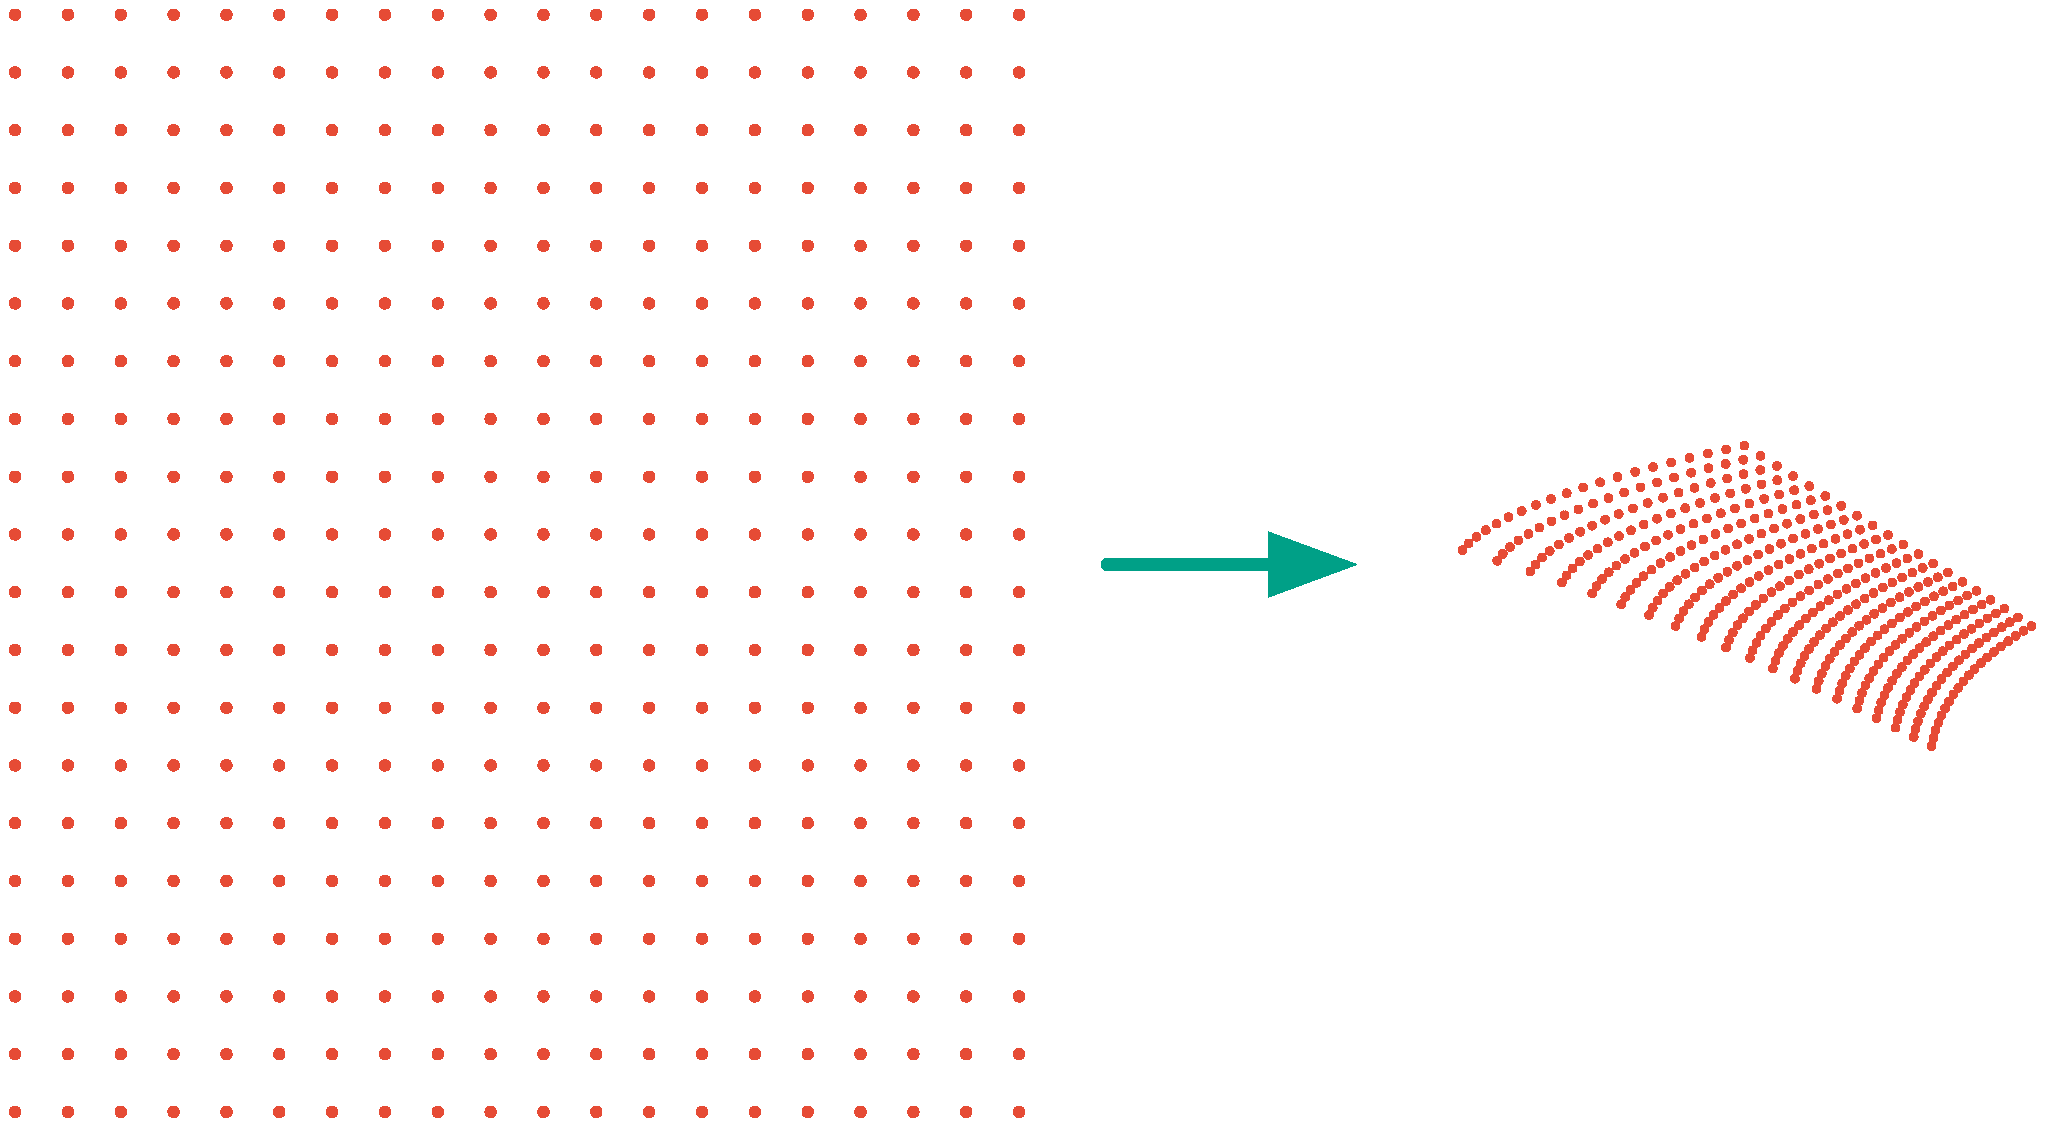
\includegraphics[width=0.7\textwidth]{src/assets/images/coords.pdf}
    \caption[Coordinates tranformation]{Transformation from visual to cortical coordinates for the 20 $\times$ 20 network.}
    \label{fig:coords-transformation}
\end{figure}
